\section{Theoretical Analysis}
\label{sec:analysis}

In this section, the circuit shown in Figure ~\ref{fig:circuit} is analysed theoretically. The following subsections correspond to the answers to the respective given exercises. 

\subsection{Task 1}

In this exercise, voltage soure $V_{S}$ is constant and it is assumed that the capacitor is constant too, which means that current $I_{c}$ is null.
Starting by calculating the voltages in evry node, we can then determine the currents in every branch using Ohm's Law (~\ref{eq:ohm_law}). 

\begin{equation}
  V= R*I.
  \label{eq:ohm_law}
\end{equation}

To calculate de voltages in every node, we labelled them with a number (see fig.~\ref{fig:circuit}). From one node to the next one we applied KCL and the given relations in the circuit shown in the introduction to calculate the seven unknown nodal voltages. We only considered nodes that do not connect to voltage sources because it decreases the complexity of the problem. 
To solve the voltages in every node and current in every branch, all the unknown currents used in the node analysis were considered to be diverging from the node. Once all the nodal voltages were calculated, everything in the circuit could be determined.

In this section we needed seven equations to determine the voltages, so we considered equations related to some nodes and added more equations derived from the analysis of the circuit. In this case, we recurred to another equation using a value $Iaux$, which is the current in the voltage source $Vd$, and an additional equation to determine de seven nodal voltages and the value of $Iaux$. Voltage in node 4 was also considered to be zero because it is connected to the ground(GND). We then solved this system of linear equations using matrixes and $Octave$. The result was the vector (V1,V2,V3,V5,V6,V7,V8,Ix). Finally, using Ohm’s Law shown in subsection 2.1 and a previous analysis, we determined the current in every branch and the values for Vb, Ib, Vc, Vd and Id (see fig.~\ref{fig:circuit}).


\begin{equation}
  V1 = Vs.
  \label{eq:n1}
\end{equation}

\begin{equation}
  (V2 - V1)*G1 + (V2 - V3)*G2 + (V2 - V5)*G3 = 0.
  \label{eq:n2}
\end{equation}

\begin{equation}
  (V3 - V2)*G2	+ (V5 - V2)*Kb = 0.
  \label{eq:n3}
\end{equation}

\begin{equation}
  (V2 - V5)*Kb + (V6 - V5)*G5 = 0.
  \label{eq:n4}
\end{equation}

\begin{equation}
  (V7 - V8)*G7 + V7*G6 = 0.
  \label{eq:n5}
\end{equation}

\begin{equation}
  (V5 - V8) + G6*Kd*V7 = 0.
  \label{eq:n6}
\end{equation}

\begin{equation}
  (V5 - V2)*G3	+ V5*G4 + (V5 - V6)*G5 - Ix = 0.
  \label{eq:n7}
\end{equation}

\begin{equation}
  Iaux = (V7 - V8)*G7.
  \label{eq:n8}
\end{equation}


These equations were computed into a matrix and solved in $Octave$ as refered before, and the values of current in every branch were calculated using Ohm's Law. The obtained results are given in Table ~\ref{tab:r1}.


\begin{table}[h]
  \centering
  \begin{tabular}{|l|r|}
    \hline    
    {\bf Name} & {\bf Voltage/Current Value}\\ \hline
    $V1$ & 5.169294e+00 \\ \hline 
$V2$ & 4.893019e+00 \\ \hline 
$V3$ & 4.311489e+00 \\ \hline 
$V5$ & 4.932163e+00 \\ \hline 
$V6$ & 5.799405e+00 \\ \hline 
$V7$ & -1.899119e+00 \\ \hline 
$V8$ & -2.873335e+00 \\ \hline 
$I1$ & 2.700573e-04 \\ \hline 
$I2$ & 2.825057e-04 \\ \hline 
$I3$ & 1.244847e-05 \\ \hline 
$I4$ & 1.206173e-03 \\ \hline 
$I5$ & 2.825057e-04 \\ \hline 
$I6$ & 9.361162e-04 \\ \hline 
$I7$ & 9.361162e-04 \\ \hline 
$Vb$ & -3.914400e-02 \\ \hline 
$Vc$ & 0.000000e+00 \\ \hline 
$Vd$ & 6.756034e-06 \\ \hline 
$Ib$ & -2.825057e-04 \\ \hline 
$Id$ & 9.361162e-04 \\ \hline 

  \end{tabular}
  \caption{Node voltages and Current in branches [A or V].}
  \label{tab:r1}
\end{table}

\newpage

\subsection{Task 2}
In this subsection, we consider until t=0, an infinite time has passed and so the capacitor is fully charged. This capacitor now functions as a voltage source $Vx$ given by the expression(\ref{eq:v_2}) as sugested. We now have a null value for $Vs$, which means it can be ignored and nodes 1 and 4 can be considered as the same, so $V1=V4=0$(GND).

\begin{equation}
  Vx = V6 - V8.
  \label{eq:v_2}
\end{equation}

The voltages $V6$ and $V8$ are the ones calculated in the previous subsection.

The main objective in this exercise is to calculate the boundary solutions, since they must be continuous, in order to calculate the equivalent resistance e the time constant for future determinations, such as the natural solution. In order to do that, we need the value $Vx$ given in the previous equation and the current that flows in between nodes 6 and 8. Using Ohm's Law, stated before, we have,

\begin{equation}
  Req = Vx/Ix.
  \label{eq:req}
\end{equation}

Once we know this value, we can now determine the time constant for the RC circuit, with the following expression,

\begin{equation}
  time constant = Req*C.
  \label{eq:tc}
\end{equation}

To obtain the value of Ix, a node analysis was necessary, similar to Exercise 1, calculating the voltages and currents in every node and branch, respectively. We needed, again, equations to then compute into a matrix and solve the linear equations system to obtain the vector (V2,V3,V5,V6,V7,V8). In this case, since the capacitor functioned as a voltage soure, we could no longer use the node analysis in node 6, but we could use it in node 4. Nodes 2,3 and 7 had no alterations, so we could use them again in this method. additional equations were added in order to solve the problem. The analysis resulted in the following expressions:


\begin{equation}
  V1 = 0.
  \label{eq:n12}
\end{equation}

\begin{equation}
  (V2 - V1)*G1 + (V2 - V3)*G2 + (V2 - V5)*G3 = 0.
  \label{eq:n22}
\end{equation}

\begin{equation}
  (V3 - V2)*G2	+ (V5 - V2)*Kb = 0.
  \label{eq:n32}
\end{equation}

\begin{equation}
  (V7 - V8)*G7 + V7*G6 = 0.
  \label{eq:n42}
\end{equation}

\begin{equation}
  V6 - V8 = Vx.
  \label{eq:n52}
\end{equation}

\begin{equation}
  (V5 - V8) + G6*Kd*V7 = 0.
  \label{eq:n62}
\end{equation}

\begin{equation}
  V2*G1 + V5*G4 + V7*G6 = 0.
  \label{eq:n72}
\end{equation}

Finally, to determine $Ix$, one can analyse node 6 with KCl:

\begin{equation}
  Ix + (V6 - V5)*G5 + Kb*(V2 - V5) = 0.
  \label{eq:Ix}
\end{equation}

The results are given in the next Table: 

 \begin{table}[h]
  \centering
  \begin{tabular}{|l|r|}
    \hline    
    {\bf Name} & {\bf Voltage/Current Value}\\ \hline
    $Vx$ & 8.672740e+00 \\ \hline 
$Ix$ & 2.825161e-03 \\ \hline 
$Req$ & 3.069821e+03 \\ \hline 
$Time Constant$ & 3.218747e-03 \\ \hline 
$V1$ & 0.000000e+00 \\ \hline 
$V2$ & 0.000000e+00 \\ \hline 
$V3$ & 0.000000e+00 \\ \hline 
$V5$ & 0.000000e+00 \\ \hline 
$V6$ & 8.672740e+00 \\ \hline 
$V7$ & 0.000000e+00 \\ \hline 
$V8$ & -0.000000e+00 \\ \hline 
$I1$ & 0.000000e+00 \\ \hline 
$I2$ & 0.000000e+00 \\ \hline 
$I3$ & 0.000000e+00 \\ \hline 
$I4$ & 0.000000e+00 \\ \hline 
$I5$ & 2.825161e-03 \\ \hline 
$I6$ & -0.000000e+00 \\ \hline 
$I7$ & 0.000000e+00 \\ \hline 
$Vb$ & -0.000000e+00 \\ \hline 
$Vd$ & 0.000000e+00 \\ \hline 
$Ib$ & -0.000000e+00 \\ \hline 
$Id$ & 0.000000e+00 \\ \hline 

  \end{tabular}
  \caption{Node voltages and Current in branches [A or V], $Req$ and $Time Constant(TC)$.}
  \label{tab:r2}
\end{table}

\newpage

\subsection{Task 3}

\par Using the results obtained in Exercise 2 for $Req$ and $Time Constant$, we can determine the natural solution:
 \begin{equation}
  V_{6n}(t) = Ae^{-\frac{t}{RC}}.
  \label{eq:v6n}
\end{equation}

\par As sugested, we used the capacitor voltage $Vx$ for $t<0$ as the initial condition. Since there is continuity, and $V6 = Vx + V8$, we have:

\begin{equation}
  V_{6n}(0) = A = V6 = Vx + V8.
  \label{eq:e31}
\end{equation}

\begin{equation}
  V_{6n}(t) = (Vx + V8)e^{-\frac{t}{RC}}.
  \label{eq:e32}
\end{equation}


\par We now have the natural solution in fuction of time for V6. With these results we were able to plot this function, as we can see in Figure \ref{fig:g_3}.

\begin{figure}[h] \centering
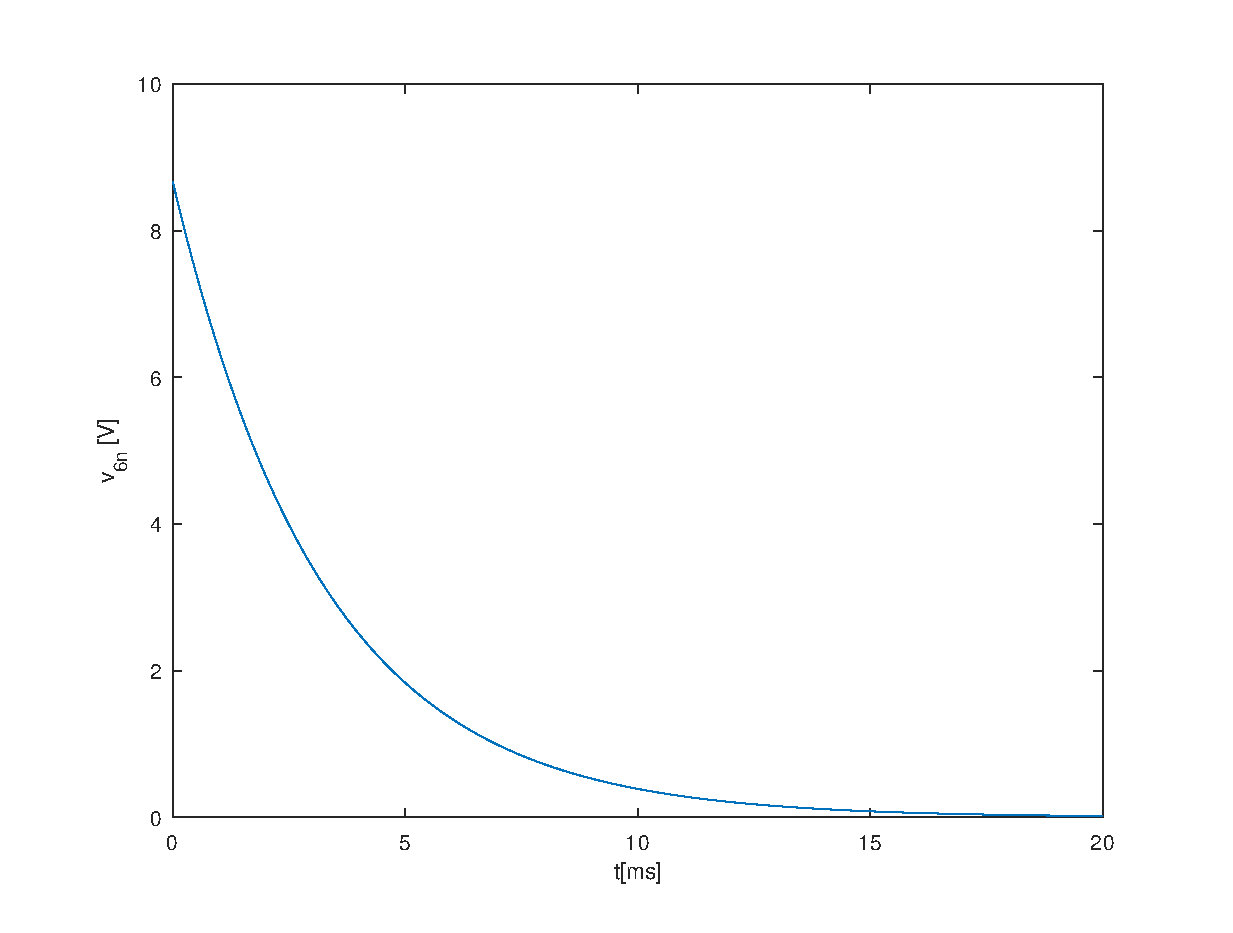
\includegraphics[width=0.8\linewidth]{natural_solution.eps}
\caption{Natural solution of V6(t) in the interval [0,20]ms.}
\label{fig:g_3}
\end{figure}
 
 \newpage
 
\subsection{Task 4}

\par In this step, the objective is to determine the forced solution for $t>0$. We now have a frequency of $f = 1KHz$, and the phasor voltage source $Vs$. The capacitor no loger functions as a voltage source. For this time interval, $Vs$ is a sinusoidal fuction of time, given by:

\begin{equation}
  Vs(t) = sin(wt).
\end{equation}

\par To simplify the problem and the calculations, we used $Vs=1V$ as sugested. We replaced C with its impedance, to determine the current

\begin{equation}
  Zc = 1/jwC.
\end{equation}

\begin{equation}
  Vc = Ic*Zc.
\end{equation}

\par Similar to before, we produced a complex node analysis (Task 1) to determine the voltage in every node. Many of the equations used in this step were derived from Task 1 (\ref{eq:n1},\ref{eq:n3},\ref{eq:n3},\ref{eq:n5},\ref{eq:n6}) and two other additional equations were added. This culminated in a matrix, that was then solved using $Octave$ maths tool.

\begin{equation}
 (V1 - V2)*G1 - G7*V5 - G6*V7 = 0.
\end{equation}

\begin{equation}
 (V6 - V5)*G5 + (V6 - V8)*Yc + (V2 - V5)*Kb = 0.
\end{equation}

\par The results are given in Table \ref{tab:t4} :

 \begin{table}[h]
  \centering
  \begin{tabular}{|l|r|}
    \hline    
    {\bf Name} & {\bf Amplitude} \\ \hline
    $V1$ & 1.000000e+00 & -5.947405e-21 \\ \hline 
$V2$ & 9.465546e-01 & 1.906228e-16 \\ \hline 
$V3$ & 8.340576e-01 & 1.644887e-14 \\ \hline 
$V5$ & 9.541270e-01 & -7.871745e-16 \\ \hline 
$V6$ & 5.579264e-01 & 1.488766e-01 \\ \hline 
$V7$ & 3.673846e-01 & -0.000000e+00 \\ \hline 
$V8$ & 5.558467e-01 & 1.597884e-15 \\ \hline 
-5.517548e-01 \\ \hline 

  \end{tabular}
  \caption{Complex analysis. Amplitude for each node.}
  \label{tab:t4}
\end{table}

\newpage

\subsection{Task 5}
In this task, to plot the graphic of the total solution, we simply summed the solutions obtained in tasks 3 and 4 (for t>=0) and used the values from task 1 when (t<0):

\begin{equation}
 V_{6t}(t) = V_{6n}(t) + V_{6f}(t).
\end{equation}

\par The plotted fuction can be seen in Figure \ref{fig:g5}.

\begin{figure}[h] \centering
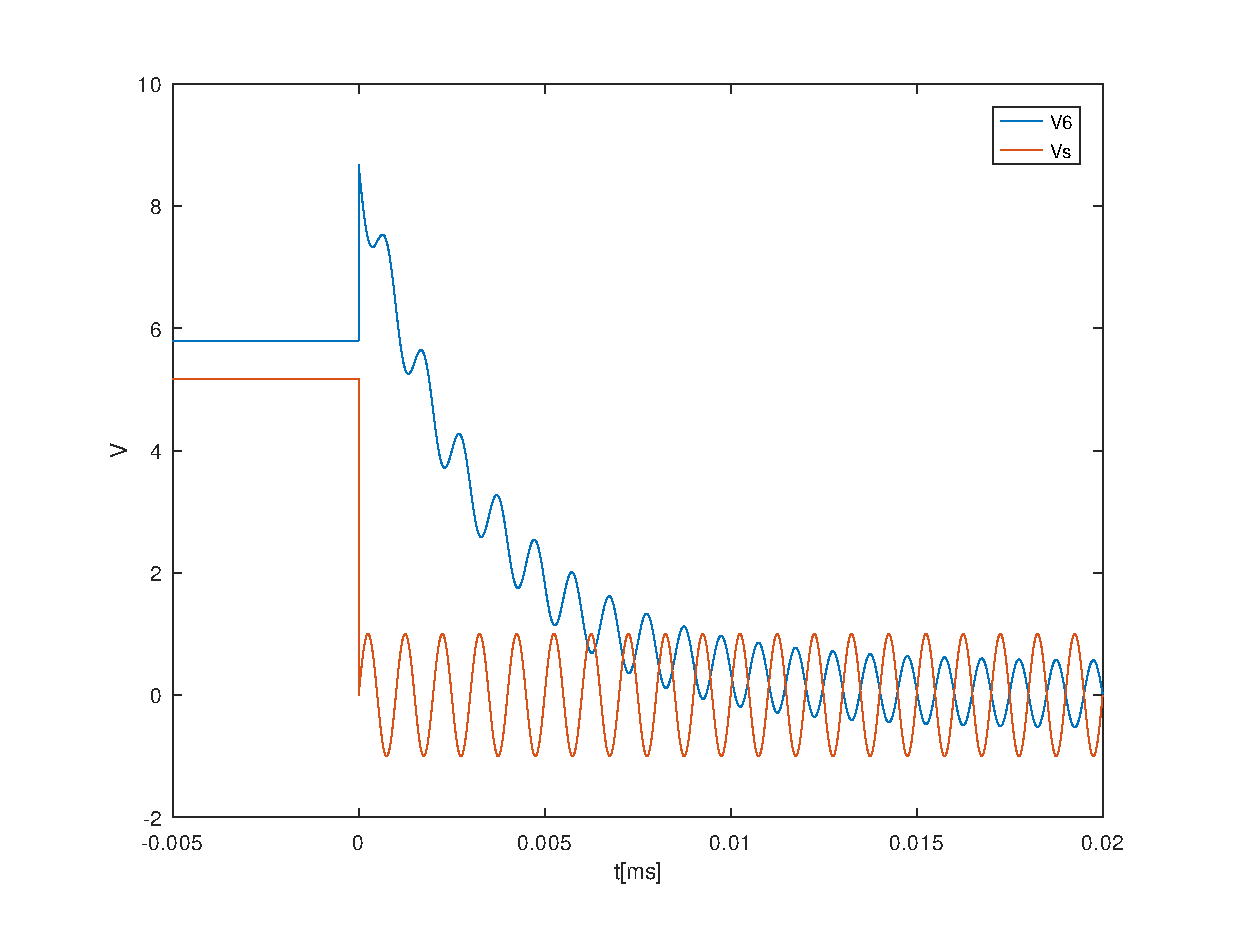
\includegraphics[width=0.8\linewidth]{tsol.eps}
\caption{Total solution of V6(t) in the interval [-5,20]ms.}
\label{fig:g5}
\end{figure}

\par These results were expected, since Vs is a voltage source and has no frequency response. Contrary, it was also expected $V6t(t)$ had a frequency response, since it depends on the voltage source. The results in the figure match the predictions.

\newpage

\subsection{Task 6}
\par In this subsection the objective was to observe the frequency responses of $Vc$ and $V6$. In order to do so we did a symilar analysis to task 4 but with a frequency vector. The values for the magnitude and phase were plotted using $Octave$. We can see the results in figures \ref{fig:g6_1} and  \ref{fig:g6_2}


\begin{figure}[h] \centering
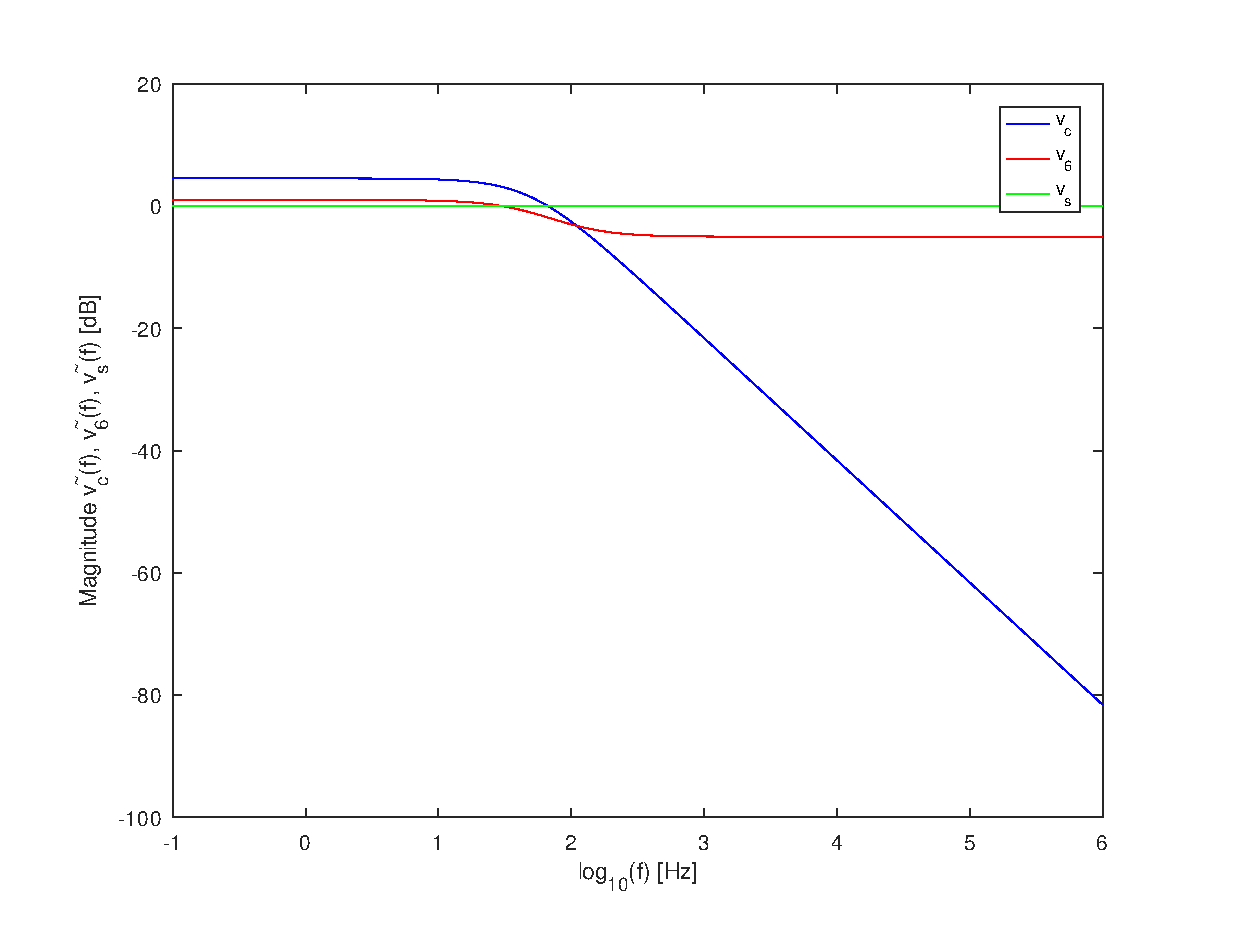
\includegraphics[width=0.8\linewidth]{magnitude.eps}
\caption{Magnitude response of Vs, V6 and Vc [dB].}
\label{fig:g6_1}
\end{figure}


\begin{figure}[h] \centering
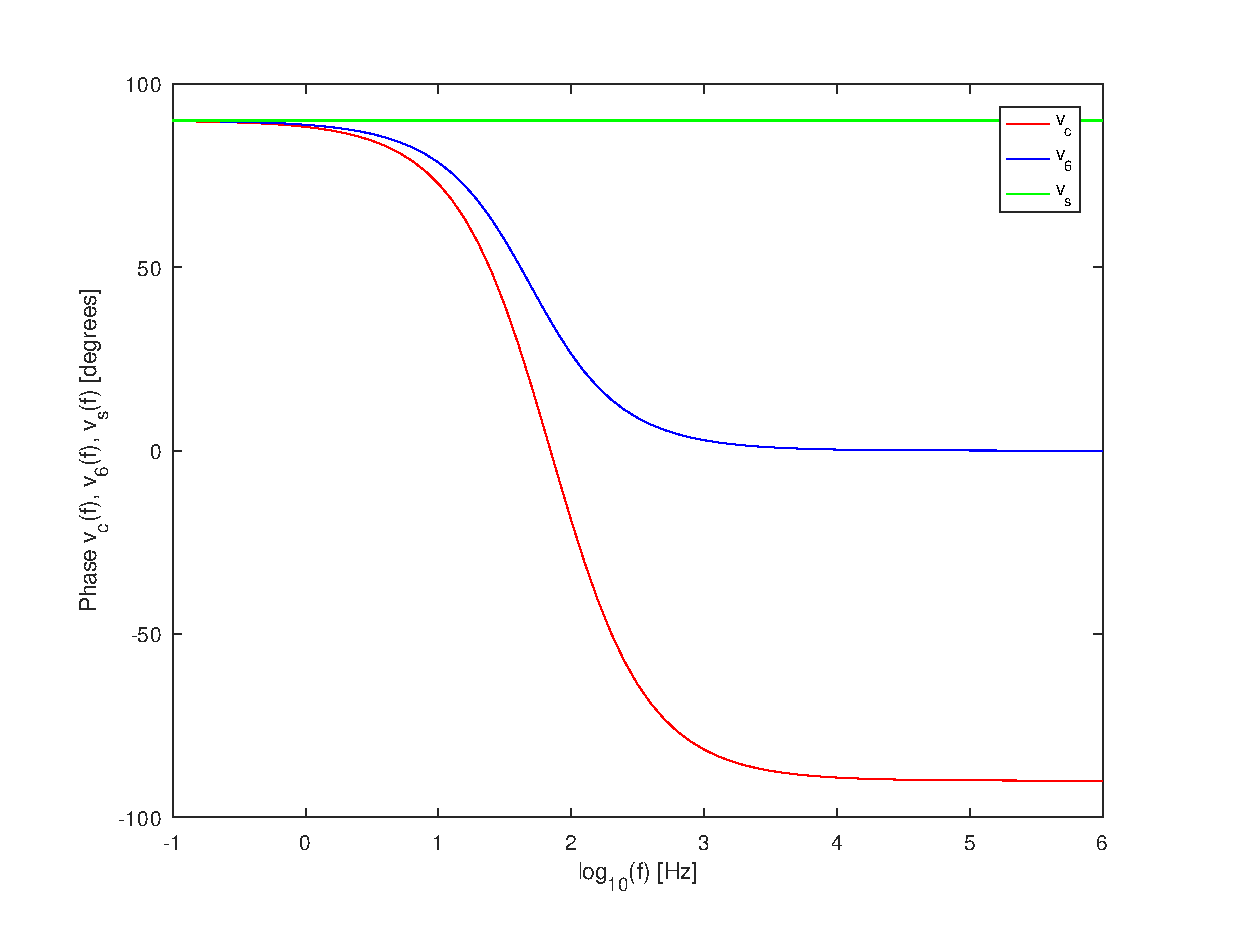
\includegraphics[width=0.8\linewidth]{phase.eps}
\caption{Angle response of Vs, V6 and Vc [degrees].}
\label{fig:g6_2}
\end{figure}

\par Looking at the plotted results, one can confirm that they match the expectations. Since we have a simple RC circuit and $Vs = 1$, we know that $Vc$ follow an inverse relation with frequency which leads us to conclude that when frequency increases, $Vc$ must decrease. Once $V8$ is a frequency independent value, one notices that $V6$ must follow the same dependence, just as we have seen in both figures.

\newpage
